\subsection{WPT metoder}
De tre relevante metoder til trådløs energi, indebære induktiv magnetisk-, resonans magnetisk kobling og mikrobølger. Induktiv og resonans virker ved near-fields og mikrobølger virker ved far-ifelds. \cite{mikro}

\begin{figure}[H]
\centering
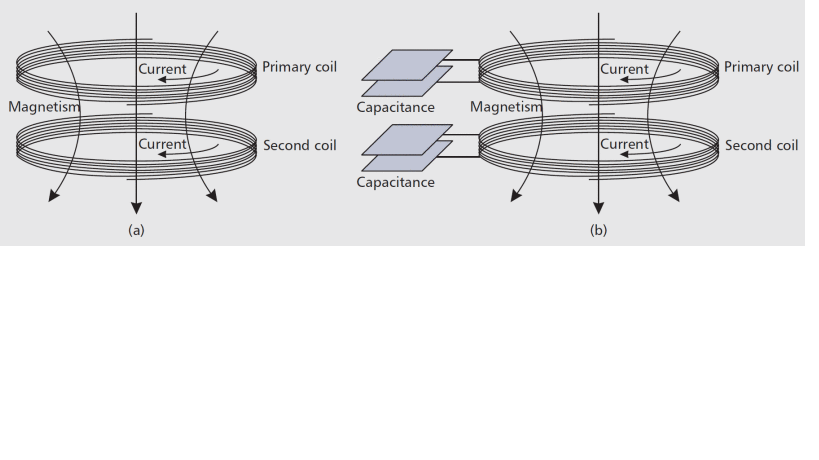
\includegraphics[scale=0.75]{Vildledning/Schematics/induktiv_resonans}
\caption{model af WPT setup \cite{mikro}}
\label{figure:wptsetup}
\end{figure}

Induktiv kobling. 
WPT ved induktiv kobling fungere, ved induktion over et magnetfelt mellem to spoler, hvilke genereres en strøm og spænding som ses på figur \ref{figure:wptsetup}a. Magnetisk induktiv kobling sker, når den primærspole som fungere som energi senderen genererer et vekselene magnetfelt på tværs af den sekundærspole, der er energien modtageren. Dette sker inden for et område generelt mindre end bølgelængden. Denne process skaber en near-field kraft, som induktiveres over den sekundære spole til en strøm/spænding, hvilket kan udnyttes af et trådløs apparatur, eksempelvis en mobil. \cite{mikro}
Fordelen ved induktiv kobling inkludere følgende; teknologien er nem, at implementer ved høj effektivitet, og det er sikkert for mennesker at være i nærheden af. Den er dog begrænset af afstand fra transmitter og receiver, idet at den har en effektiv energioverførelse mellem nogle få millimeter til et par centimeter. Ulemper ved induktiv kobling indebære den relative korte ladeafstand, varmen der udvikles i spolerne, og spolerne skal ligge meget tæt for, at kunne opnå den maksimale effekt.
Teknologien bliver i dag set i mobile enheder (mobiltelefoner og tablets), tandbørster, RFID-tags, induktionskomfur og betalingskort. \cite{mikro}

Resonant kobling. 
Magnetisk resonant kobling er baseret på kortvarige bølgekobling, hvilke genere og overføre en elektrisk strøm mellem to resonante spoler i et oscillerende eller varierende magnetfelt, som set på figur \ref{figure:wptsetup}b. Da de to spoler køre på samme resonant frekvens, kan der opnå en høj effektiv elektrisk energioverførelse, med meget lidt tab til  eksterne faktorer. Denne indskab gøre energioverførelsen næsten upåvirket af omgivelserne, hvilke også gør det muligt at lade selvom der er noget i mellem transmitter og receiver. 
Den klare fordel ved resonans kobling er den meget større effektive lade distance, som kan opnå en effekt på 90 procent optil 1 meter mellem transmitter og receiver, og 40 procent ud til to meter. \cite{mikro} Derudover kan en enkel transmitter lade flere receivere på samme tid så længe de operer på sammen resonans frekvens.
En af ulemperne ved resonant kobling er at hver receiver kræver en dedikeret kapacitets spole, hvilke gøre det svært at gøre receiveren lille nok til mobile enheder, og det gøre det generelt mere kompliceret at implementere. \cite{mikro}